\documentclass[9pt,aspectratio=1610]{beamer}

\usepackage{color,fancybox,alltt,graphicx}

\usepackage{pgf,pgfarrows,pgfnodes,pgfautomata,pgfheaps,pgfshade}

\usepackage[latin1]{inputenc}
\usepackage{colortbl}
\usepackage[english]{babel}
\usepackage{multimedia}
\usepackage{amssymb,amsmath}
\usepackage{ragged2e}
\usepackage{animate}
\usepackage{listings}

\newif\ifpdf
\ifx\pdfoutput\undefined
\pdffalse % we are not running PDFLaTeX
\else
\pdfoutput=1 % we are running PDFLaTeX
\pdftrue
\fi

\mode<article>{ \usepackage{fullpage}  \usepackage{pgf}  \usepackage{hyperref} }


\mode<presentation>{
  \usetheme{XAFS}
  \setbeamercovered{transparent}
}

\usepackage{amsmath}
\usepackage{tikz}

\usepackage[customcolors,shade]{hf-tikz}

\usetikzlibrary{calc}

% put color to \boxed math command
\newcommand*{\cmboxcolor}{orange}
\makeatletter
\newcommand{\cmbox}[1]{\textcolor{\cmboxcolor}{%
 \makeatother
\tikz[baseline={([yshift=-1ex]current bounding box.center)}] \node [rectangle, minimum width=1ex,rounded corners,draw] {\normalcolor\m@th$\displaystyle#1$};}}



\usepackage[latin1]{inputenc}
\usepackage[english]{babel}
\setbeamertemplate{navigation symbols}{}

\setlength{\fboxrule}{1pt}


\newcommand{\vmm}{{\vspace{2mm}}}
\newcommand{\hmm}{{\hspace{1mm}}}
\newcommand{\Justify}{\justify\vspace{-\baselineskip}}

\newcommand{\Program}[1]{\scshape{#1}}
\newcommand{\atoms}{{\Program{atoms}}}
\newcommand{\feffit}{{\Program{feffit}}}
\newcommand{\ifeffit}{{\Program{ifeffit}}}
\newcommand{\larch}{{\Program{larch}}}
\newcommand{\xasviewer}{{\Program{XAS Viewer}}}

\newcommand{\ease}{{\Program{EASE}}}
\newcommand{\autobk}{{\Program{autobk}}}
\newcommand{\ffchi}{{\Program{ff2chi}}}
\newcommand{\diffkk}{{\Program{diffkk}}}
\newcommand{\sixpack}{{\Program{sixpack}}}
\newcommand{\hephaestus}{{\Program{hephaestus}}}
\newcommand{\athena}{{\Program{athena}}}
\newcommand{\artemis}{{\Program{artemis}}}
\newcommand{\feff}{{\Program{feff}}}
\newcommand{\mxan}{{\Program{mxan}}}
\newcommand{\fdmnes}{{\Program{fdmnes}}}
\newcommand{\gnuplot}{{\Program{gnuplot}}}

\newcommand{\file}[1]{{{\slshape\ttfamily{#1}}}}
\newcommand{\feffndat}{\file{feffnnnn.dat}}
\newcommand{\feffbin}{\file{feff.bin}}


\newcommand{\bmu}{{\mu}}
\newcommand{\bepsilon}{{\epsilon}}
\newcommand{\bDelta}{{\Delta}}
\newcommand{\bOmega}{{\Omega}}
\newcommand{\bdelta}{{\delta}}
\newcommand{\bsigma}{{\sigma}}
\newcommand{\bln}{{\ln}}
\newcommand{\bsum}{{\sum}}
\newcommand{\bsim}{{\sim}}
\newcommand{\bsin}{{\sin}}
\newcommand{\bexp}{{\exp}}
\newcommand{\bint}{{\int}}
\newcommand{\bpsi}{{\psi}}
\newcommand{\bpropto}{{\propto}}
\newcommand{\bapprox}{{\approx}}
\newcommand{\bchi}{{\chi}}
\newcommand{\brho}{{\rho}}
\newcommand{\bpi}{{\pi}}
\newcommand{\balpha}{{\alpha}}
\newcommand{\bbeta}{{\beta}}
\newcommand{\blambda}{{\lambda}}
\newcommand{\blesssim}{{\lesssim}}
\newcommand{\brightarrow}{{\rightarrow}}
\newcommand{\bAA}{{\rm\AA}}
\newcommand{\mbf}[1]{{\ensuremath{\mathbf\mathit{#1}}}}

\newcommand{\chie}{{\ensuremath{\chi(E)}}}
\newcommand{\chik}{{\ensuremath{\chi(k)}}}
\newcommand{\chir}{{\ensuremath{\chi(R)}}}
\newcommand{\mue}{{\ensuremath{\mu(E)}}}
\newcommand{\bkg}{{\ensuremath{\mu_0(E)}}}

\definecolor{lightyellow}{rgb}{1.0,1.0,0.8}
\definecolor{lightyellow2}{rgb}{1.0,1.0,0.97}
\definecolor{golden}{rgb}{0.75,0.75,0.37}
\definecolor{lightpink}{rgb}{1.0,0.9,0.9}
\definecolor{nearwhite}{rgb}{0.95,0.94,0.94}
\definecolor{verywhite}{rgb}{0.99,0.99,0.99}
\definecolor{white}{rgb}{1.0,1.0,1.0}
\definecolor{DarkBlue}{rgb}{0,0,0.3}
\definecolor{BrightBlue}{rgb}{0,0,0.7}
\definecolor{DarkRed}{rgb}{0.65,0,0}
\definecolor{BrightRed}{rgb}{0.8,0,0}
\definecolor{RRed}{rgb}{0.95,0,0}
\definecolor{BlueGrey}{rgb}{0.2,0.1,0.1}

\definecolor{VBlue}{rgb}{0,0,0.9}
\definecolor{BrightGreen}{rgb}{0,0.6,0.0}
\definecolor{DarkGreen}{rgb}{0,0.3,0}


\newcommand{\Color}[2]{{\textcolor{#1}{#2}}}
\newcommand{\Red}[1]{{\Color{BrightRed}{#1}}}
\newcommand{\RRed}[1]{{\Color{RRed}{#1}}}
\newcommand{\DarkRed}[1]{{\Color{DarkRed}{#1}}}
\newcommand{\Blue}[1]{{\Color{BrightBlue}{#1}}}
\newcommand{\BrightBlue}[1]{{\Color{BrightBlue}{#1}}}
\newcommand{\Black}[1]{{\Color{black}{#1}}}
\newcommand{\RedM}[1]{{\Color{red}{\mbf{#1}}}}
\newcommand{\BlueM}[1]{{\Color{blue}{\mbf{#1}}}}
\newcommand{\BlackM}[1]{{\Color{black}{\mbf{#1}}}}


\newcommand{\DarkGreen}[1]{{\Color{DarkGreen}{#1}}}
\newcommand{\DarkBlue}[1]{{\Color{DarkBlue}{#1}}}


\newcommand{\RedEmph}[1]{{\Color{BrightRed}{\emph{#1}}}}
\newcommand{\RedSl}[1]{{\Color{BrightRed}{\slshape{#1}}}}
\newcommand{\BlueSl}[1]{{\Color{BrightBlue}{\slshape{#1}}}}
\newcommand{\BlueEmph}[1]{{\Color{BrightBlue}{\emph{#1}}}}


\newcommand{\LString}[1]{{\Color{BrightGreen}{{#1}}}}
\newcommand{\LKeyword}[1]{{\Color{DarkRed}{{#1}}}}
\newcommand{\LFunc}[1]{{\Color{VBlue}{{#1}}}}
\newcommand{\LComment}[1]{{\Color{BrightRed}{{#1}}}}


\newcommand{\pthpar}[1]{{\ensuremath{{\tt{\Blue{#1}}}}}}

\newcommand{\feffc}[1]{{{\ensuremath{{\Red{#1}}}}}}
\newcommand{\reff}{{{\feffc{R_{\rm eff}}}}}
\newcommand{\twothirds}{{{\textstyle{2 \over 3}}}}
\newcommand{\fourthirds}{{{\textstyle{2 \over 3}}}}
\newcommand{\masse}{{({{2m_e} / {\hbar^2}})}}

\newcommand{\highlightbox}[1]{{ \fcolorbox{black}{lightyellow}{#1}}}

\newenvironment{VerbSBox}[1]%
{\VerbatimEnvironment\begin{Sbox}%
\begin{minipage}{#1}\begin{alltt}}%
{\end{alltt}\end{minipage}\end{Sbox}\setlength{\fboxsep}{2mm}{%
\begin{flushright}\shadowbox{\TheSbox}\end{flushright}}}
%%

\newenvironment{VerbSSBox}[1]%
{\VerbatimEnvironment\begin{Sbox}%
\begin{minipage}{#1}\begin{alltt}}%
{\end{alltt}\end{minipage}\end{Sbox}\setlength{\fboxsep}{2mm}{%
\begin{center}\shadowbox{\TheSbox}\end{center}}}
%%

% \newenvironment{VerbBox}[1]%
% {\VerbatimEnvironment\begin{Sbox}%
% \begin{minipage}{#1}\begin{alltt}}%
% {\end{alltt}\end{minipage}\end{Sbox}\setlength{\fboxsep}{2mm}{%
% \shadowbox{\TheSbox}
% %%

\newenvironment{CodeBlock}[2]%
{\VerbatimEnvironment\begin{minipage}{#1}\begin{block}{\small{#2}}\begin{semiverbatim}\tiny}%
{\end{semiverbatim}\end{block}\end{minipage}}%%

\definecolor{DeepGrey}{rgb}{0.15,0.05,0.05}
\newcommand{\GreyLine}{{\color{DeepGrey}{\rule{\linewidth}{1.00pt}}}}

\newcommand{\STitle}[1]{{\hspace{2mm}{\bfseries\sl\Large%
      \BrightBlue{#1}}}\hfill\par%
  \vspace{-3.5mm}\GreyLine\vspace{-0.1mm}}

\newenvironment{ListingBlock}[2]%
{\begin{minipage}{#1}\begin{block}{\small{#2}}\begin{lstlisting}}
{\end{lstlisting}\end{block}\end{minipage}}%%

\newenvironment{figblock}[3]%
{\begin{minipage}{#1}\begin{exampleblock}{#2}{\wgraph{#1}{#3}}}%
{\end{exampleblock}\end{minipage}}%

\newenvironment{MFrame}[1]%%
{\subsection{#1}\begin{frame}\frametitle{#1}}%
{\end{frame}}%

\newenvironment{Boxedminipage}%
    {\begin{Sbox}\begin{minipage}}%
    {\end{minipage}\end{Sbox}\shadowbox{\TheSbox}}


\setbeamercolor{postit}{fg=black,bg=lightyellow}

\newenvironment{postitbox}[1]%%
{\begin{center}\begin{minipage}{#1}\begin{beamercolorbox}[shadow=true,rounded=true]{postit}}%
{\end{beamercolorbox}\end{minipage}\end{center}}%


\newenvironment{postitboxC}%%
{\begin{center}\begin{beamercolorbox}[center,shadow=true,rounded=true]{postit}}%
{\end{beamercolorbox}\end{center}}%

\newcommand{\entrylabel}[1]{ {\Blue{#1:}}}
%%\newcommand{\entrylabel}[1]{{\parbox[b]{10mm}{%
%%      \makebox[10mm][l]{{\Red{#1:}}}\\}}}

\newenvironment{entry}
{\begin{list}{}{\renewcommand{\makelabel}{\entrylabel}%
      \setlength{\labelwidth}{7mm}
      \setlength{\leftmargin}{6mm}}}{\end{list}}

\newcommand{\redlabel}[1]{ {\Color{DarkRed}{#1}}}
\newenvironment{redlist}[1]{\begin{list}{}{\renewcommand{\makelabel}{\redlabel}%
      \setlength{\leftmargin}{#1}}}{\end{list}}


\newcommand{\bluelabel}[1]{ {\Color{BrightBlue}{#1}}}
\newenvironment{bluelist}[1]{\begin{list}{}{\renewcommand{\makelabel}{\bluelabel}%
      \setlength{\leftmargin}{#1}}}{\end{list}}

\newcommand{\xbluelabel}[1]{{\Color{BrightBlue}{#1\hspace{2mm}}}}
\newenvironment{xbluelist}[1]{\begin{list}{}{\renewcommand{\makelabel}{\xbluelabel}%
      \setlength{\leftmargin}{#1}}}{\end{list}}

\newenvironment{cenpage}[1]%%  centered minipage
{\begin{center}\begin{minipage}{#1}}%
    {\end{minipage}\end{center}}%%

\newenvironment{slide}[1]%%  begin named slide
{\begin{frame}\frametitle{#1}}%
{\end{frame}}%%

\newenvironment{fslide}[1]%%  begin named slide
{\subsection{#1}\begin{frame}[fragile]\frametitle{#1}}%
{\end{frame}}%%


\newcommand{\xdgraph}[2]{{%
        \ifpdf  \includegraphics[width={#1}]{figs/#2.png}%
        \else   \includegraphics[width={#1}]{figs/#2.eps}\fi}}

\newcommand{\rgraph}[2]{\includegraphics[width={#1}]{figs/rimg/#2}}
\newcommand{\wgraph}[2]{\includegraphics[width={#1}]{figs/#2.png}}
\newcommand{\hgraph}[2]{\includegraphics[height={#1}]{figs/#2.png}}
\newcommand{\wpdf}[2]{\includegraphics[width={#1}]{#2.pdf}}

\newcommand{\webpage}[1]{{{\Blue{{#1}}}}}

%% \pgfdeclareimage[interpolate=true,width=45mm]{xafscartoon}{figs/xafsabsorb}
%% \pgfdeclareimage[interpolate=true,width=50mm]{xafsxanes}{figs/xafsxanes}
%% \pgfdeclareimage[interpolate=true,width=50mm]{feff}{figs/scattamp}
%% \pgfdeclareimage[interpolate=true,width=55mm]{tdlplot}{figs/tdlplot}

%% \pgfdeclareimage[interpolate=true,width=15mm]{ravel}{figs/RavelHead}
%% \pgfdeclareimage[interpolate=true,width=15mm]{calvin}{figs/CalvinHead}
%% \pgfdeclareimage[interpolate=true,width=15mm]{frenkel}{figs/FrenkelHead}
%% \pgfdeclareimage[interpolate=true,width=15mm]{haskel}{figs/HaskelHead}
%% \pgfdeclareimage[interpolate=true,width=15mm]{jox}{figs/JoxHead}
%% \pgfdeclareimage[interpolate=true,width=15mm]{newville}{figs/NewvilleHead}
%% \pgfdeclareimage[interpolate=true,width=15mm]{kelly}{figs/KellyHead}

%% \pgfdeclareimage[interpolate=true,width=15mm]{rehr}{figs/RehrHead}
%% \pgfdeclareimage[interpolate=true,width=15mm]{fons}{figs/FonsHead}
%% \pgfdeclareimage[interpolate=true,width=15mm]{webb}{figs/WebbHead}
%% \pgfdeclareimage[interpolate=true,width=15mm]{glover}{figs/GloverHead}
%% \pgfdeclareimage[interpolate=true,width=15mm]{trainor}{figs/TrainorHead}

%% \pgfdeclareimage[interpolate=true,width=85mm]{APS2005_Photo}{figs/APS2005_Photo}

%% \pgfdeclareimage[interpolate=true,width=68mm]{EASE}{figs/EASE}

\begin{document}


\title[Virtual XAFS School]{Using FEFF for EXAFS Data Analysis}  %%  and FEFF fitting}
\author[M Newville]{Matthew Newville}
\date{July-2021}

\institute[Univ of Chicago]{Center for Advanced Radiation Sources\\
  The University of Chicago}

\begin{frame} \titlepage
  \vmm
  \begin{center}
    Fundamentals of X-ray Absorption Fine-Structure
  \end{center}

  \vmm

  \begin{cenpage}{60mm}
    Virtual XAFS School at Illinois Institute of Technology and Advanced
  Photon Source
\end{cenpage}
\end{frame}

\section{The EXAFS Equation (REVIEW)}

\section{The EXAFS Equation}

\begin{slide}{The EXAFS Equation}  % XAFS Analysis with {\feff}}

  \begin{cenpage}{135mm}

  The XAFS Equation used with {\feff}:

  \[
  \chi(k) = \sum_j {{ S_0^2 {\Blue{N_j}} {\Red{f_j(k)}}  e^{-2R_j/{\Red{\lambda(k)}}}
      e^{-2k^2{\Blue{\sigma_j^2}}}}\over{k{\Blue{R_j}}^2}}
  {\sin[{2k{\Blue{R_j}} + {\Red{\delta_j(k)}}} ]}
   \]

   \begin{itemize}
  \item $\Red{f(k)}$ and $\Red{\delta(k)}$ are  {\emph{photo-electron scattering
        amplitude and phase}}:
    \begin{itemize}
    \item Energy dependent    \hspace{3mm}  $k \sim \sqrt{(E-E_0)} $.
    \item Depend on $Z$ of the scattering atom(s).
    \item Non-trivial: must be calculated or carefully extracted from  measured spectra.
    \end{itemize}

\item $\Red{\lambda(k)}$ tells how far the photo-electron can travel.

\item The sum is over {\RedEmph{Scattering Paths}} of the photo-electron,
  from absorbing atom to neighboring atom(s) and back.  May include
  {\BlueEmph{multiple scattering}}!

\end{itemize}

   \onslide+<2->

   \begin{postitbox}{64mm}
     If we know $\Red{f(k)}$,  $\Red{\delta(k)}$, and $\Red{\lambda(k)}$, we can get:
     \begin{itemize}
     \item ${\Blue{R}}$ --  near neighbor distance.
     \item ${\Blue{N}}$ -- coordination number.
     \item ${\Blue{\sigma^2}}$ -- mean-square  disorder in ${\Blue{R}}$.
     \end{itemize}
   \end{postitbox}

\end{cenpage}  \end{slide}

\section{{\feff}}


\subsection{Scattering Amplitude and Phase}


\begin{slide}{Scattering Amplitude and Phase-Shift: ${f(k)}$ and ${\delta(k)}$ }

  \begin{cenpage}{135mm}

  The scattering amplitude ${\Red{f(k)}}$ and phase-shift
  ${{\Red{\delta(k)}}}$ depend on Z:

    \vmm

    \begin{tabular}{ll}
      \begin{minipage}{55mm}
        \rgraph{55mm}{scatt_amp}
        \end{minipage} &
        \begin{minipage}{55mm}
          \rgraph{55mm}{scatt_pha}
      \end{minipage}\\

      \begin{minipage}{55mm}
      $\Red{f(k)}$ peaks at higher  $k$ as Z increases.  Heavy
        elements, have a characteristic dip in $\Red{f(k)}$, and
        scatter to high $k$.

        {\bf{Note: O is done at $k>15\rm\AA^{-1}$}}


      \end{minipage}
      &
      \begin{minipage}{55mm}

        The phase shift $\Red{\delta(k)}$ also shows strong Z
        dependence, and has sharp jumps for heavy elements where $f(k)$ dips.

        {\bf{Note:  $\delta(k) \approx -k$! }}
      \end{minipage} \\
    \end{tabular}

\begin{postitbox}{50mm}
  Z can usually be determined to $\pm 5$.

\vmm
  Fe and O can be distinguished.

\vmm
  N  and O cannot be distinguished.
\end{postitbox}
\vfill

\end{cenpage}  \end{slide}


\begin{slide}{ $\lambda(k)$: The Photo-Electron Mean-Free Path }

  \begin{cenpage}{135mm}

  The $ e^{-2R/\lambda(k)} $ term in the XAFS Equation accounts for how far the
   photo-electron can travel and still return (in phase) to the excited atom.
 \begin{columns}
   \begin{column}{55mm}
     \rgraph{57mm}{lambda}
   \end{column}
   \begin{column}{60mm}

     This includes both:

     \begin{itemize}
     \item  inelastic scattering of photo-electron.
     \item  finite lifetime of the core-hole (fs).
     \end{itemize}
     \vmm

   \end{column}
 \end{columns}

 \vmm\hrule\vmm

The photo-electron goes only {10 to 20 \AA}  over most of the EXAFS region.

 \begin{postitbox}{80mm}
     The $\lambda$ and $1/R^{2}$ terms make EXAFS a  {\RedEmph{local probe}}.
   \end{postitbox}

 \end{cenpage}  \end{slide}



\begin{slide}{EXAFS Analysis Strategy:  How to get $N$, $R$, etc?}

  \begin{cenpage}{135mm}

    % \begin{center}\begin{minipage}[t][12mm]{90mm}
      \[
      \chi(k) = \sum_j {{ S_0^2 {\Blue{N_j}} {\Red{f_j(k)}}  e^{-2R_j/\lambda(k)}
          e^{-2k^2{\Blue{\sigma_j^2}}}}\over{k{\Blue{R_j}}^2}}
      {\sin[{2k{\Blue{R_j}} + {\Red{\delta_j(k)}}} ]}
      \]
   %% \end{minipage}  \end{center}

   \vmm
   Steps:
   \begin{enumerate}
   \item Calculate theoretical XAFS spectra  with {\feff},  starting with a guess of the local structure.
   \item  {\RedEmph{Refine}} $R$, $N$, and $\sigma^2$  to best match  experimental data.
   \item Compare lots of refined models.
   \end{enumerate}

\vmm \vmm \hrule \vmm\vmm

 Questions you might have (and we might answer!):

  \begin{itemize}
  \item How do we run {\feff} to generate $\Red{f(k)}$, $\Red{\delta(k)}$,
    and  $\Red{\lambda(k)}$?
  \item What correction factors do we need to worry about?
  \item How do we fit experimental data?
  \item How do we interpret the results?
  \item Any advice for making all this, um, easier?
  \end{itemize}

\vfill
\end{cenpage}  \end{slide}


\subsection{{\feff}}
\begin{slide}{{\feff} Calculation Overview: What does {\feff} do? }

  \begin{cenpage}{135mm}

  {\feff} calculates the EXAFS {$\chi(k)$}  by simulating the scattering of a
  photo-electron along all scattering paths from a selected absorbing atom within
  a  cluster of atoms.

    \vmm

  \begin{enumerate}
    \onslide+<1->\item   build atomic potentials.   To  simplify calculations,
      \begin{center}
        \begin{tabular}{ll}
          \begin{minipage}{75mm}
            Use the {\BlueEmph{Cup-Cake Tin Approximation}}:
            atomic potentials up to a uniform Fermi level -no chemical bonding.

            \hspace{2mm}(Some people call this ``Muffin-Tin'' Approximation)
          \end{minipage}
          &
          \begin{minipage}{30mm}
            \vspace{1mm} 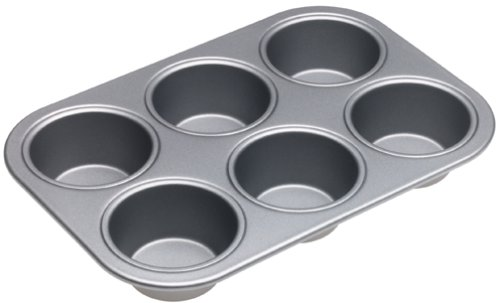
\includegraphics[width=27mm]{figs/theory/muffintin2}
          \end{minipage}
        \\
      \end{tabular}
    \end{center}


  \onslide+<2->\item determine important scattering paths.

    \begin{itemize}
    \item Build paths from a selected {\BlueEmph{central atom}} in a cluster of atoms
    \item decide which ones are ``degenerate'' (=``'equivalent'',   !=``degraded state'')
    \item decide which ones are unimportant for XAFS
    \end{itemize}


  \onslide+<3->\item move photo-electron along path to determine
    $\Red{f}$ and $\Red{\delta}$ as a function of $k$:

    \begin{center}
      propagate $\Rightarrow$ scatter $\Rightarrow$ propagate $\Rightarrow$ \ldots.
    \end{center}

  \end{enumerate}

\end{cenpage}  \end{slide}

\subsection{{\feff}   complications}
\begin{slide}{{\feff}: what's so hard about that??}

  \begin{cenpage}{135mm}

    {\feff} includes sophisticated techniques to calculate of \feffc{f(k)},
    \feffc{\delta(k)}, and \feffc{\lambda(k)}.

    \begin{description}
    \item[\RedEmph{Curved Wave Effects}] the photo-electron goes out as
      spherical wave and scatters from atoms with finite size.

    \item[\RedEmph{Muffin-Tin Approximation:}] Makes the calculations
      tractable, but is an approximation.

    \item[\RedEmph{Multiple Scattering}]  the photo-electron can scatter
      multiple times. Most important at low $k$ and for \BlueEmph{linear paths}.

    \item[\RedEmph{Extrinsic Losses}] {\feffc{\lambda(k)}}: self-energy and
      core-hole lifetime.

    \item[\RedEmph{Intrinsic Losses}] {\feffc{S_0^2}}: the absorbing atom
      relaxes to the presence of the hole left in the core electron level.

    \item[\RedEmph{Polarization Effects}] synchrotron beams are highly
      polarized, which needs to be taken into account.  This is simple for
      $K$ edges ($s\rightarrow p$ is dipole), but slightly more complicated for
      $L$ and $M$ edges.

    \end{description}

\vmm
\begin{center} Usually, you don't have to worry about these things.\end{center}

\end{cenpage}  \end{slide}


\section{{\feff} complications}

\subsection{{\feff} complication \#1: Multiple Scattering}

\begin{slide}{{\feff} complication \#1: Multiple Scattering}

  \begin{cenpage}{135mm}

  \vmm
\begin{columns}
  \begin{column}{50mm}
  The photo-electron can scatter multiple times before getting back to the
  absorbing atom:

  \begin{center}
    \rgraph{50mm}{mspaths}
  \end{center}

  \end{column}
  \begin{column}{60mm}

  A {\Blue{Path Formalism}} is used in the  calculation:

  \begin{center}
    propagate $\Rightarrow$ scatter $\Rightarrow$ propagate $\Rightarrow$ \ldots.
  \end{center}

  \vmm
  \vmm {\Red{Single Scattering}}  usually important.

  \vmm {\Red{Triangle Paths}} with angles $ 45 < \theta <
  135^{\circ}$ scatter weakly, but there are lots of them.

  \vmm {\Red{Linear paths}} with angles $\theta \approx 180^{\circ}$
   are very strong: the photo-electron is {\Red{focused}} through an atom.
   Can be used to measure bond angles\ldots

  \end{column}
  \end{columns}

   \begin{postitbox}{92mm}
     \Red{ A {\feff} Path looks the same for Single and Multiple
       Scattering}
   \end{postitbox}
\end{cenpage}  \end{slide}

\subsection{{\feff} Complication \#2: S02}
\begin{slide}{{\feff} complication \#2: $S_0^2$, the  Amplitude Reduction Term}

  \begin{cenpage}{135mm}

  \vmm
  The {\RedEmph{other}} electrons in the absorbing atom can relax due to
  the core-hole, giving an {\Red{Amplitude Reduction Term}}:

   \vmm
   \[
   S_0^2 =  {  |{\langle \Phi^{N-1}_f |\Phi^{N-1}_0 \rangle}|^2}
   \]

    \vspace{1mm}

    ${| \Phi^{N-1}_0 \rangle }$ = $(N-1)$ electrons in unexcited atom.

    ${\langle \Phi^{N-1}_f|}$   = $(N-1)$ electrons, relaxed by core-hole.

    \vmm

    \onslide+<2->
    ${S_0^2}$ is taken as a constant: \hspace{3mm}  $ 0.7 < S_0^2 < 1.0 $.

    and may be used as a Fitting Parameter that multiplies {$\chi$}:

    \vmm \vmm
    \begin{center}
      {\Red{ ${S_0^2}$ is Completely Correlated with $N$      (!!!)}}
    \end{center}


    \begin{postitbox}{68mm}
      $S_0^2$ is usually constant for  data measured on
      the same edge {\bf{and}} beamline (energy resolution).
    \end{postitbox}

    Most Common Approach: Determine $S_0^2$ from experimental data on a
    system with known $N$, and then use that for unknown data.

    \vmm

  \end{cenpage}  \end{slide}

\section{Practical FEFF}

\begin{slide}{ Practical {\feff} }

    \begin{cenpage}{110mm}

{\RedEmph{Good News}}: you don't have to worry about the hard parts (mostly)!

\begin{enumerate}
\item Start with a structure close to the {\BlueEmph{local}} atomic structure
  of your sample, and generate x,y,z coordinates for the atoms. Often a
  crystal structure is close -- it does not have to be perfect!

\item Run {\feff}.  This creates a {\feffndat} files for each path.

\item Use these  Path Files in to model measured XAFS.
\end{enumerate}

  {\larch} and {\xasviewer} helps you find crystal structures, create and
  edit input filess, run {\feff}, and sort and use the results. 

\begin{columns}
      \begin{column}[T]{88mm}
        \begin{block}{ run {\feff} in a specified folder  }
          \begin{semiverbatim} {\footnotesize larch>
{\LFunc{feff8l}}({\LString{'feff8.inp'}}, folder={\LString{'CuS\_Feff'}}) }
          \end{semiverbatim}
        \end{block}

      \end{column}
      \begin{column}[T]{1mm} \end{column}
    \end{columns}


\end{cenpage}

  Having good starting structures can be important, but you do not need the
  exact structure to use {\feff}.

\vmm


  You can (may need to) mix structural models to model real data.

\end{slide}{

\subsection{Anatomy of {\file{feff.inp}}}
\begin{frame}[fragile] \frametitle{Anatomy of {\file{feff.inp}}}

\begin{cenpage}{100mm}
  {\feff} is a very old program that runs from an input file -- it
  {\bf{must}} be called {\file{feff.inp}}.   {\larch} can help with this.
  \vmm

  Each calculation should be in its own folder/subdirectory.
\end{cenpage}


\begin{tabular}{lr}
  \begin{CodeBlock}{48mm}{\file{feff.inp} file ({\feff} 8):}
{\Blue{TITLE    FeO, rock salt structure}}
{\Blue{EDGE K}}
{\Blue{S02   1.0}}
{\Blue{CONTROL  1 1 1 1 1 1}}  {\Red{\# which parts of code to run}}
{\Blue{PRINT    1 0 0 0 0 3}}  {\Red{\# which output files to write}}
{\Blue{RPATH   6.0}}   {\Red{\# How far in R to build paths}}

{\Blue{POTENTIALS }}      {\Red{\# list of Atomic Potentials}}
* potential  z  label
      0     26  Fe   {\Red{\# Absorbing Atom}}
      1      8  O    {\Red{\# 1 Potential for each Z}}
      2     26  Fe

{\Blue{ATOMS}}  {\Red{\# list of Atomic X, Y, Z, Potential }}
 0.00000     0.00000     0.00000    0   Fe
 0.00000     0.00000    -2.13870    1   O
-2.13870     0.00000     0.00000    1   O
 0.00000    -2.13870     0.00000    1   O
 0.00000     0.00000     2.13870    1   O
 2.13870     0.00000     0.00000    1   O
 0.00000     2.13870     0.00000    1   O
 0.00000     2.13870     2.13870    2   Fe
 0.00000    -2.13870    -2.13870    2   Fe
\end{CodeBlock} &
\begin{minipage}{67mm}

\onslide<2->

{\file{feff.inp}} includes:

\vmm

\begin{enumerate}
  \onslide<2->\item A list of unique Atomic Potentials:
  \begin{itemize}
  \item 1 Absorbing Atom, always Potential 0 
  \item 1 Potential per atomic species (Z)
  \end{itemize}

  \onslide<2->\item List of atomic coordinates (in {\AA}):

  {\hmm\hmm}  $x$, $y$, $z$, $Pot$

  for each atom in the cluster of atoms 

  \vmm
  The cluster can be non-crystalline.

  \vmm
  The absorber can be at (0, 0, 0), or not.

  \vmm
  Hint:  better off removing H atoms!

\end{enumerate}
\end{minipage}\\
\end{tabular}

  \onslide<2->
   \begin{postitbox}{90mm}
     \Red{You can edit the atomic positions, and add or change potentials.}
   \end{postitbox}

\end{frame}


\begin{slide}{Input Parameters for {\file{feff.inp}  ({\feff} 8)}}

\begin{cenpage}{100mm}
  {\feff} has many  inputs, but only a few of them are really
  important for EXAFS Analysis (some are {\Red{\texttt{required}}}, some {\Blue{\texttt{optional}}}):

  \begin{description}[POTENTIALSXX]
  \item[{\Red{\texttt{EDGE}}}]   which edge  absorbs  the x-ray ({\tt{K}}, {\tt{L3}}, etc.)

  \item[{\Red{\texttt{POTENTIALS}}}]   list of atomic potentials (0 = absorbing atom)

  \item[{\Red{\texttt{ATOMS}}}]   list of atomic $x$, $y$, $z$, Potential

  \item[{\Red{\texttt{CONTROL}}}]   which ``Modules'' to run.  Use  ``1 1 1 1 1 1''.

  \item[{\Red{\texttt{PRINT}}}]   which ``Outputs'' to write. Use  ``1 0 0  0 0 3''.


  \item[{\Blue{\texttt{RPATH}}}]   how far out (in {\AA}) to consider the  cluster of atoms.

  \item[{\Blue{\texttt{POLARIZATION}}}]   polarization vector of incident
    x-ray (in same coordinate system as atomic coordinates)

  \item[{\Blue{\texttt{EXCHANGE}}}]   which model to use for the exchange energy.
    Use the default (Hedin-Lundqvist model) unless you know why.

  \end{description}

\end{cenpage}

\end{slide}



\subsection{ Converting CIF data into {\feff} inputs}
\begin{frame}[fragile] \frametitle{Converting CIF data into {\feff} inputs}

\begin{cenpage}{95mm}

  {\larch} comes with about 9000 crystral structures from the 

\end{cenpage}

  \begin{cenpage}{75mm}
    American Mineralogist Crystal Structure Database 
  \end{cenpage}

\begin{cenpage}{95mm}


  and can convert these as {\RedEmph{Crystallographic Information Format}}
  (CIF) files to {\feff} input files.

  \vmm
  It handles fractional site occupancy with weighted substitutions -- use
  with caution!

  \vmm
  It can also read some CIF files from other sources (work-in-progress!).

  \vmm
  This is a convenient way to generate a {\feff} input, but not necessary!

\begin{postitbox}{84mm}
  The cluster used by {\feff} does not need to be a crystal!
\end{postitbox}

\vmm
Atomic clusters may also come from:

\vmm
Protein Data Bank, Molecular Dynamics Simulations, 
Density Functional Theory Calculations, \ldots.


\end{cenpage}
\end{frame}


\begin{slide}{{\feff}:  what {\em{should}} you worry about?}

  Using {\feff} in a real analysis, we'll be {\BlueEmph{refining}}
  bond lengths and coordination numbers.  For this to work, here are some
  ``rules of thumb'':

  \begin{cenpage}{90mm}

\begin{enumerate}
   \item refining distances by {\bf{more than $0.1\rm\,\AA$}} probably means
  the calculation should be re-run -- the overlap of atomic potentials may
  not be accurate.

   \item  refining energy origins $E_0$ by {\bf{more than $10\rm\,eV$}} may
  mean the calculation -- or the selection of $E_0$ in the data reduction
  -- is wrong or needs to be re-examined.

 \item  {\feff} can set $S_0^2$ and make a simple attempt at
  $\sigma^2$ values.  {\bf{don't use these}}.

 \item You {\bf{should set $S_0^2$}} for a particular group
  of data (central atom, beamline energy resolution, etc), based on an
  experimental standard, or have uncertain values for $N$.
  \end{enumerate}
  \end{cenpage}

\end{slide}

\section{XAFS Analysis -- Data Modeling}

\subsection{Path Parameters}
\begin{frame}
\frametitle{XAFS Analysis with  {\larch} and {\feff}}

To model XAFS as a Sum of Paths:

\[
\chi(k) = \sum_j {{{\Blue{S_0^2 N_j}} {\Red{f_j(k)}}  e^{-2R_j/\lambda(k)}
    e^{-2k^2{\Blue{\sigma_j^2}}}}\over{k{\Blue{R_j}}^2}}
{\sin[{2k{\Blue{R_j}} + {\Red{\delta_j(k)}}} ]}
\]

we may refine these Parameters {\RedEmph{For Each Path}}:

\begin{center}
  \begin{tabular}{lll}
    In XAFS           &  {\larch}     &  Physical \\
    Equation         &  Parameter  & Meaning \\
    \noalign{\hrule} \noalign{\smallskip}
    $N S_0^2 $     & {\tt{s02}}    &  Amplitude Factor:   $N$ and $ S_0^2$ \\
    $E_0$             & {\tt{e0}}     &  Energy Shift (where $k=0$) \\
    $\Delta R$     & {\tt{deltar}}   &  Change in path length $R = \Delta R + R_{\rm  eff}$ \\
    $\sigma^2 $  & {\tt{sigma2}} &  Mean-square-displacement in  $R$ \\
    \noalign{\hrule}
  \end{tabular}
\end{center}


\begin{itemize}

\item $R_{\rm eff}$ is the starting $R$ value for the {\feff} Path.

\item Other Parameters: higher order cumulants, energy broadening, \ldots

\item In principle, any parameter for any path could be refined.

\end{itemize}


\end{frame}


\begin{frame}
\frametitle{EXAFS Analysis: Modeling the 1st Shell of FeO}

\begin{cenpage}{135mm}
    \begin{columns}
      \begin{column}{80mm}
        FeO has a rock-salt structure.
        \vmm\vmm

        To model the Fe $K$ edge EXAFS of FeO, we'll calculate the
        {\file{feffNNNN.dat}} files (with ${{\Red{f(k)}}}$ and
        ${{\Red{\delta(k)}}}$), for Fe-O based on the FeO crystal
        structure.

        \vmm

        We'll then  {\BlueEmph{refine}} the values
        {\Blue{${R}$}}, {\Blue{${N}$}},
        {\Blue{${\sigma^2}$}}, and {\Blue{${E_0}$}} so our
        model EXAFS function matches our data.
        \vspace{2mm}

      \end{column}
      \begin{column}{25mm}

         \wgraph{24mm}{molecules/feo}

         Fe-O octahedra, ${R=2.14\rm\,\AA}$.

    \end{column}
    \end{columns}

    \onslide+<2->

    \begin{columns}
      \begin{column}{65mm}

        \vspace{-3mm}
        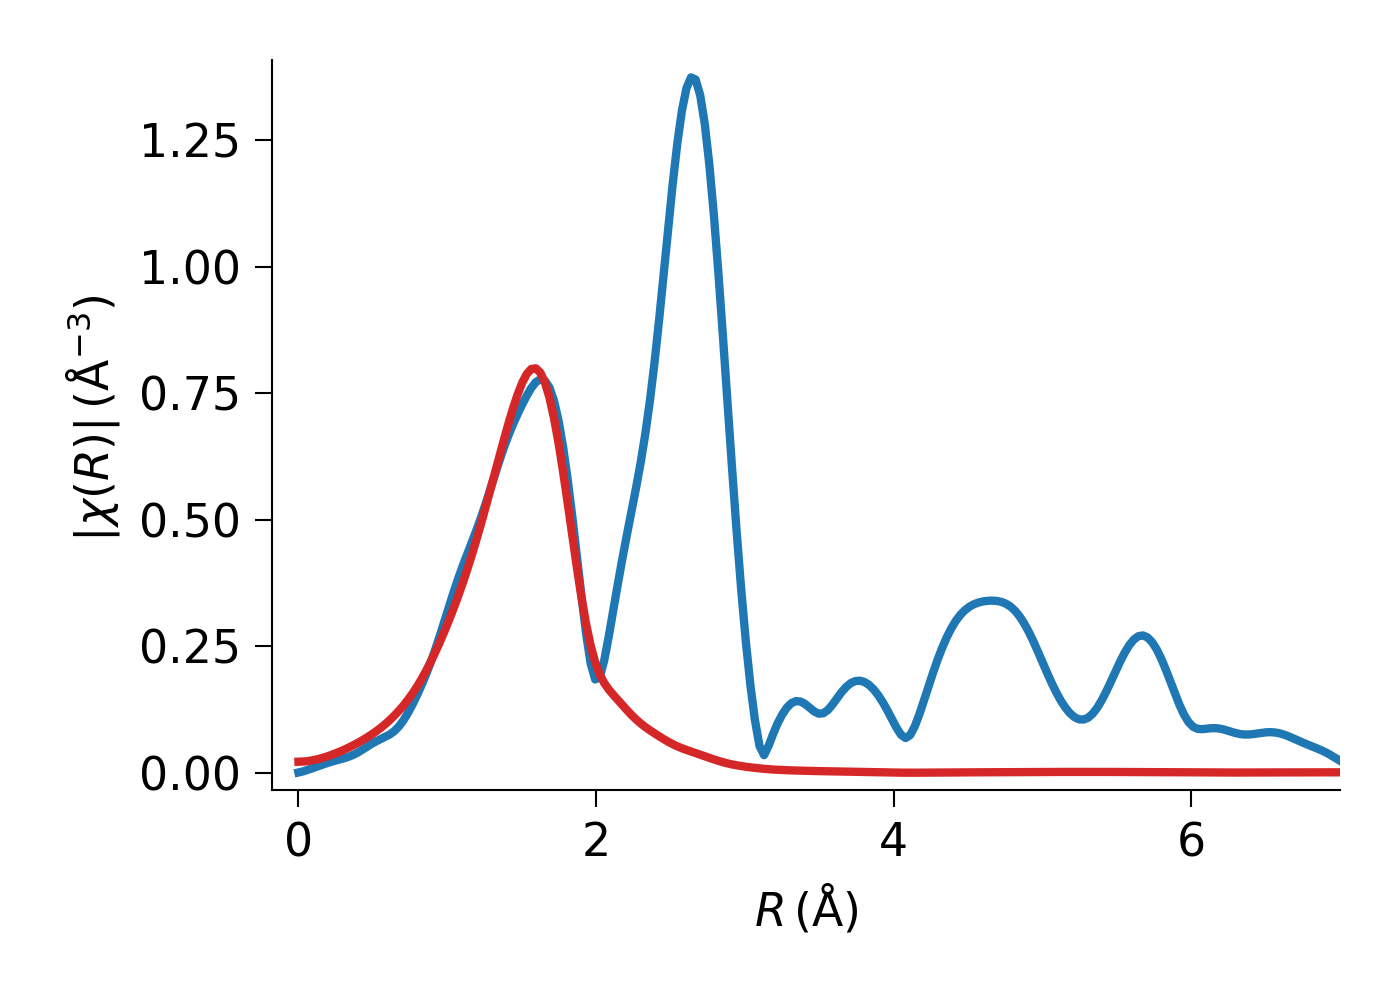
\includegraphics[width=63mm]{figs/fits/feo_1sh_chirmag}

        \vmm
        ${|\chi(R)|}$ for FeO {\Blue{data}} and {\Red{${\rm 1^{st}}$ shell
            fit}}.

      \end{column}
      \begin{column}{35mm}\onslide+<2->
        \setlength{\baselineskip}{10pt} \vmm
        Results:   \vmm
        \begin{tabbing}[ll]\= aaaaa\= aaaaaaaaaaaaaaaa\kill
          \> ${S_0^2}$     \>= 0.7 (fixed)\\
          \> ${N}$           \>= 5.1 ${\pm}$ 0.4\\
          \> ${R}$           \>= 2.09 ${\pm}$ 0.01\AA\\
          \> ${\Delta E_0}$ \>= -1.3 ${\pm}$ 0.9 eV\\
          \> ${\sigma^2}$   \>= 0.012 ${\pm}$ 0.002
          ${\rm\,\AA^2}$.\\
          \end{tabbing}

        \vfill
    \end{column}
  \end{columns}

  \vfill
  \end{cenpage}
\end{frame}

\begin{frame}
\frametitle{Analysis Example:  1st Shell of FeO}
  \begin{cenpage}{135mm}
    \begin{tabular}{ll}
      \begin{minipage}{65mm}
        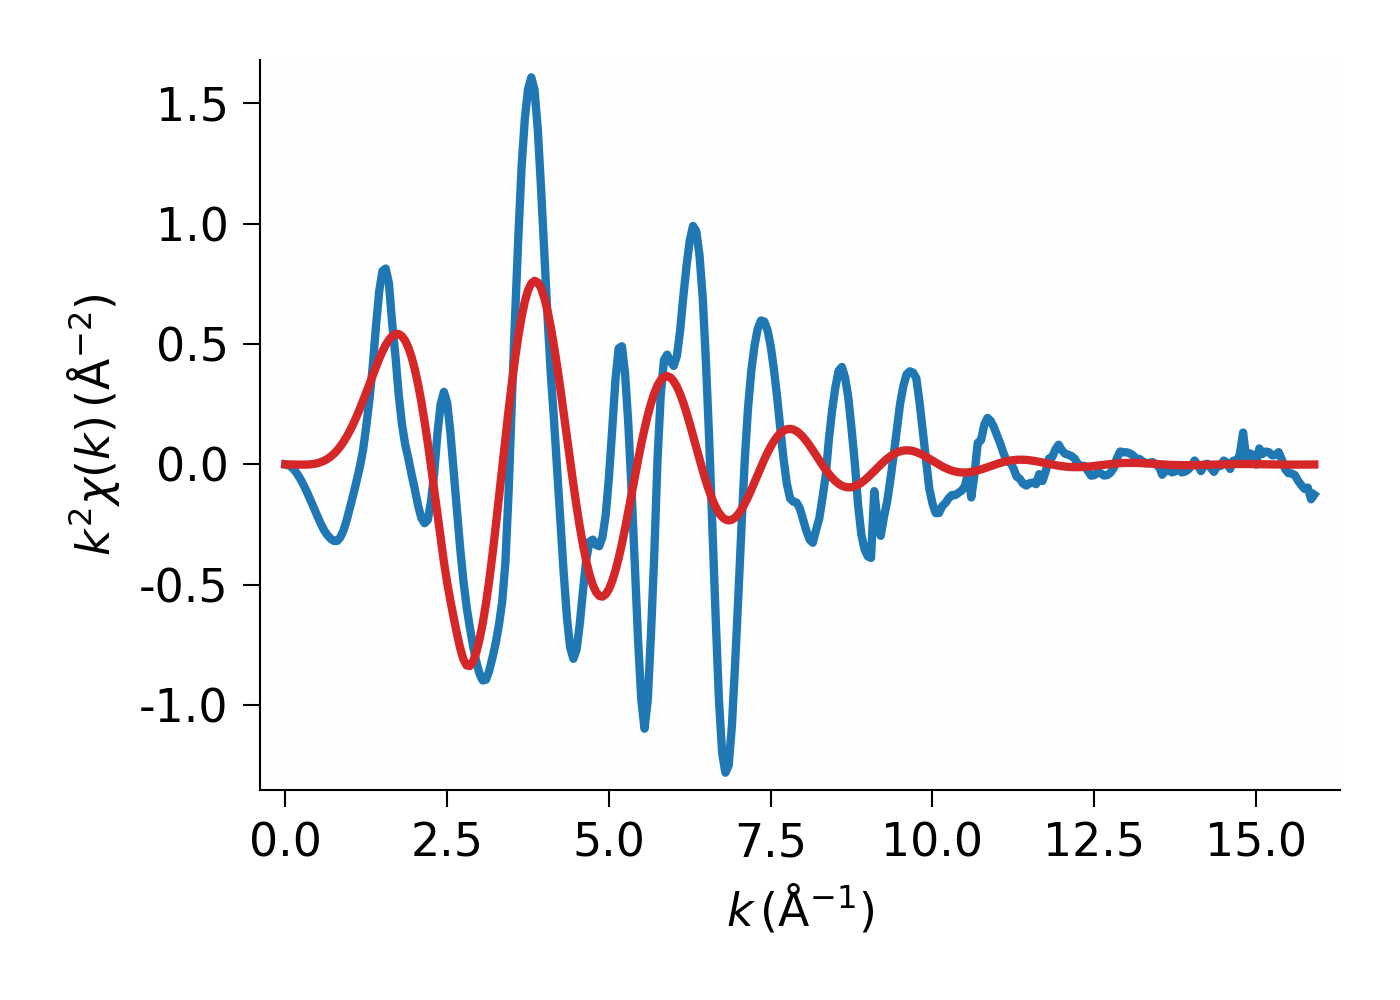
\includegraphics[width=63mm]{figs/fits/feo_1sh_chik}
      \end{minipage}
      &
      \begin{minipage}{55mm}  \setlength{\baselineskip}{10pt}

        {\Red{${1^{st}}$ shell fit in ${k}$ space.}}
        \vmm

        There is clearly another component in the XAFS!
        \vfill
      \end{minipage}
    \\
    \onslide+<2->
      \begin{minipage}{65mm}
        \vspace{-3mm}
        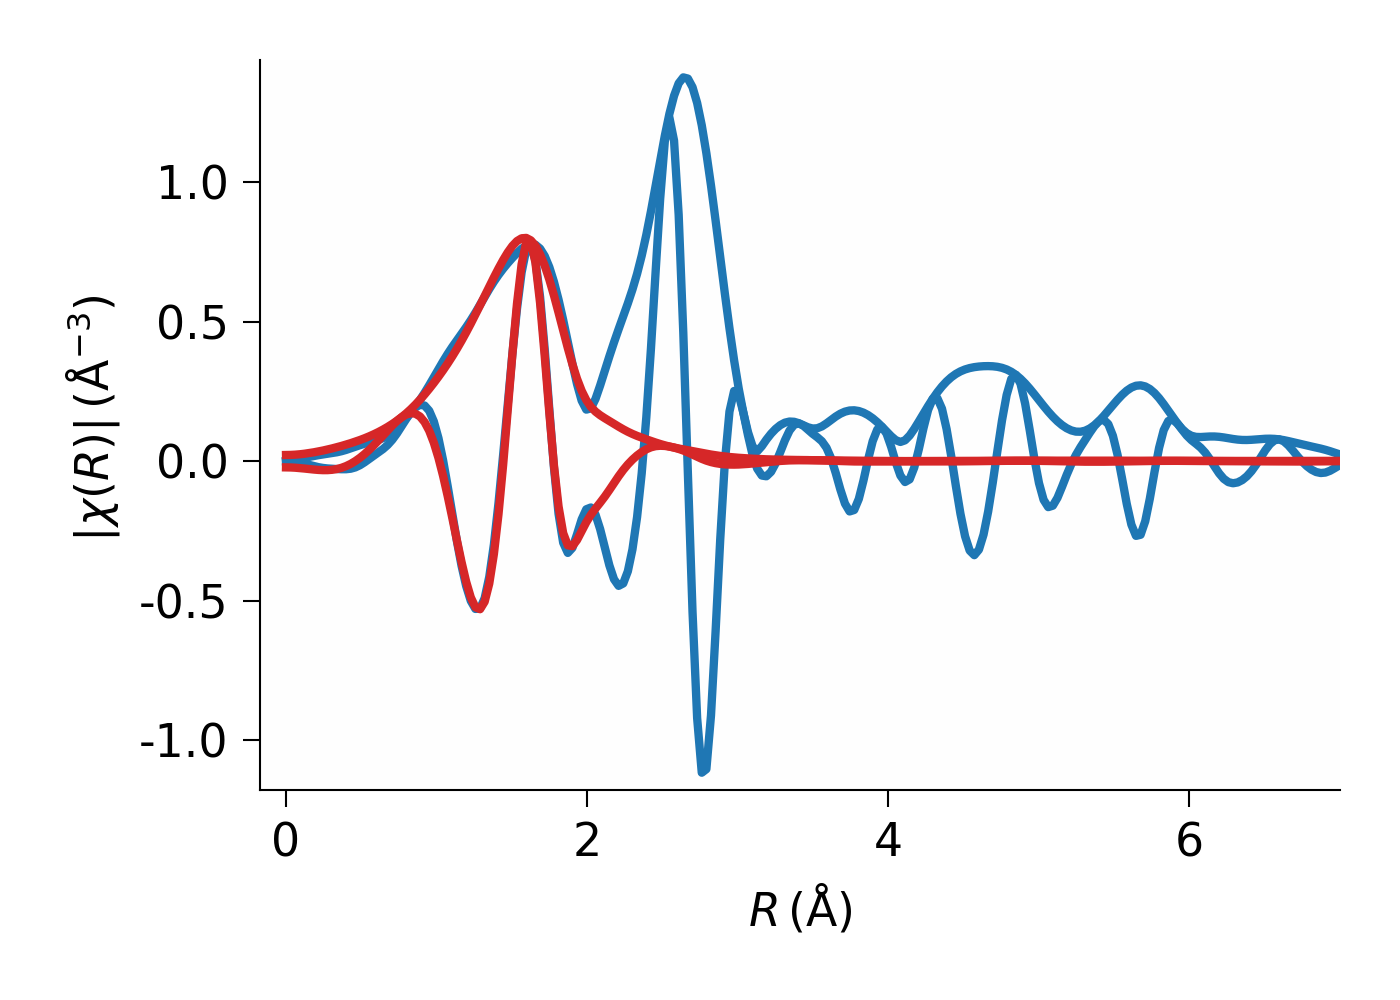
\includegraphics[width=63mm]{figs/fits/feo_1sh_chirre}
      \end{minipage}
      &
    \onslide+<2->
      \begin{minipage}{55mm}  \setlength{\baselineskip}{10pt}
        {\Red{${1^{st}}$ shell fit in ${R}$ space.}}
        \vspace{1mm}

        ${|\chi(R)|}$ and
        {\BlueEmph{${\rm Re[\chi(R)]}$}} for
          FeO (blue), and a ${\rm 1^{st}}$ shell fit (red).  \vspace{1mm}

        Though the fit to the magnitude isn't perfect,
        the fit to ${\rm Re[\chi(R)]}$ looks very good.
        \vfill
      \end{minipage}
  \end{tabular}

  \vfill
    \end{cenpage}
\end{frame}


% \section{Fitting Data}

\begin{slide}{Fitting Strategies}

  Data analysis seeks a {\RedEmph{Model}} that best matches a
  {\BlueEmph{Measurement}}.

  \vmm

  We'll use $\chi^2$ (don't confuse with EXAFS $\chi$!!) to describe how
  good the match is:

  \[ \chi^2  =
  \sum_i^{N_{\rm fit}} \frac{[\chi_i^{\rm measured} - \chi_i^{\rm
      model}({x})]^2}{\epsilon^2}
  \]

  where
  \begin{itemize}
  \item $N_{\rm fit} = $ number of points in the data to fit.
  \item $\epsilon = $ the  estimated noise  level in the data.
  \item $x$  is the set of parameters to be varied in the analysis
  \end{itemize}

  \begin{center}
    {\RedEmph{ The Best Fit is the one with lowest $\chi^2$. }}
  \end{center}

  \vmm   \hrule \vmm

  \onslide+<2->

  Questions:

  \begin{enumerate}
  \item How do I know how many independent measurements I have?
  \item What is $\epsilon$ for my data?
  \item What parameters can/should I vary?
  \end{enumerate}

\end{slide}

\begin{slide}{The Information Content of EXAFS}

\begin{cenpage}{105mm}
    The number of parameters we can reliably extract from our data is limited:
    \vspace{1mm}


    \begin{postitbox}{26mm}
      $\displaystyle  N_{\rm idp} \approx { \frac{2 \Delta k \Delta R}{\pi}}  $
    \end{postitbox}

    \vmm

    where $\Red{ \Delta k}$ and $\Red{ \Delta R}$ are the $k$- and
    $R$-ranges of the usable data.

    \onslide+<2->
    \vmm\vmm

    For a typical range of $k = [3.0, 12.5] \rm\,\AA^{-1}$ and $R = [1.0,
    3.0] \rm\,\AA$, there are $\sim 12$ parameters that can be determined
    from EXAFS.      \onslide+<2-> That's not much!

    \onslide+<2->
    \vmm\vmm

    The Fit statistics and confidence in the measured parameters need to
    reflect this.  But we usually oversample our data ($N_{\rm fit} >
    N_{\rm idp} $) so we have

    \begin{postitbox}{56mm}
      $ \displaystyle
      \chi^2  =  \frac{ N_{\rm idp}}{\epsilon^2 N_{\rm fit}}
      \sum_i^{N_{\rm fit}} [\chi_i^{\rm measured} - \chi_i^{\rm model}({x})]^2
      $
    \end{postitbox}

    Note: I also assumed $\epsilon$ is a constant.

\vfill
\end{cenpage}
\end{slide}


\begin{slide}{Other Fitting Statistics}

  Other ``goodness-of-fit statistics'':
  \vmm

  {\RedEmph{chi-square}}: As before:

  \begin{postitbox}{54mm}  $ \displaystyle
    \chi^2  =  \frac{ N_{\rm idp}}{\epsilon^2 N_{\rm fit}}
    \sum_i^{N_{\rm fit}} [\chi_i^{\rm measured} - \chi_i^{\rm model}({x})]^2
    $
  \end{postitbox}

 \vmm
  {\RedEmph{reduced chi-square}}: scale $N_{\rm varys}$ by the ``degrees of freedom'' :

  \begin{postitbox}{38mm}
    $ \chi^2_\nu =  \chi^2 / (N_{\rm idp}-N_{\rm varys}) $
  \end{postitbox}


  For a ``Good Fit'', $\chi^2_\nu$ should be $\sim$ 1.   This
  {\RedEmph{never}} happens!

\vmm

  {\RedEmph{R-factor}}: $\cal{R}$  gives a ``fractional misfit'' (and
  not scaled by the data  uncertainty $\epsilon$):

\vmm

  \begin{postitbox}{50mm}
    \[
{\cal{R}} = \frac{\sum_i^{N_{\rm fit}}[\chi_i^{\rm measured} -
      \chi_i^{\rm model}({x})]^2 }{
      \sum_i^{N_{\rm fit}} [{\chi_i^{\rm measured}}]^2}
    \]
  \end{postitbox}

\vfill

\end{slide}

%%%%%%%%%%%%%%%%%%%%%%


\section{Uncertainties in $\chi(k)$}
\begin{frame}\frametitle{Propagation of uncertainties in $\chi(k)$}

\begin{cenpage}{95mm}

  Estimating uncertainties in  $\chi(k)$ has always been a challenge.

  \vmm

  We have (by default) estimated the uncertainty in $\chi(k)$ as
  {\BlueEmph{white noise}} {\tiny{(Newville, Boyanov, and Sayers, {\emph{J
          Synch Rad}}, 1999)}}, using $\chi(R)$ between [15, 25] \AA.

\end{cenpage}

\begin{columns}
  \begin{column}[T]{60mm}

    {\onslide+<1->  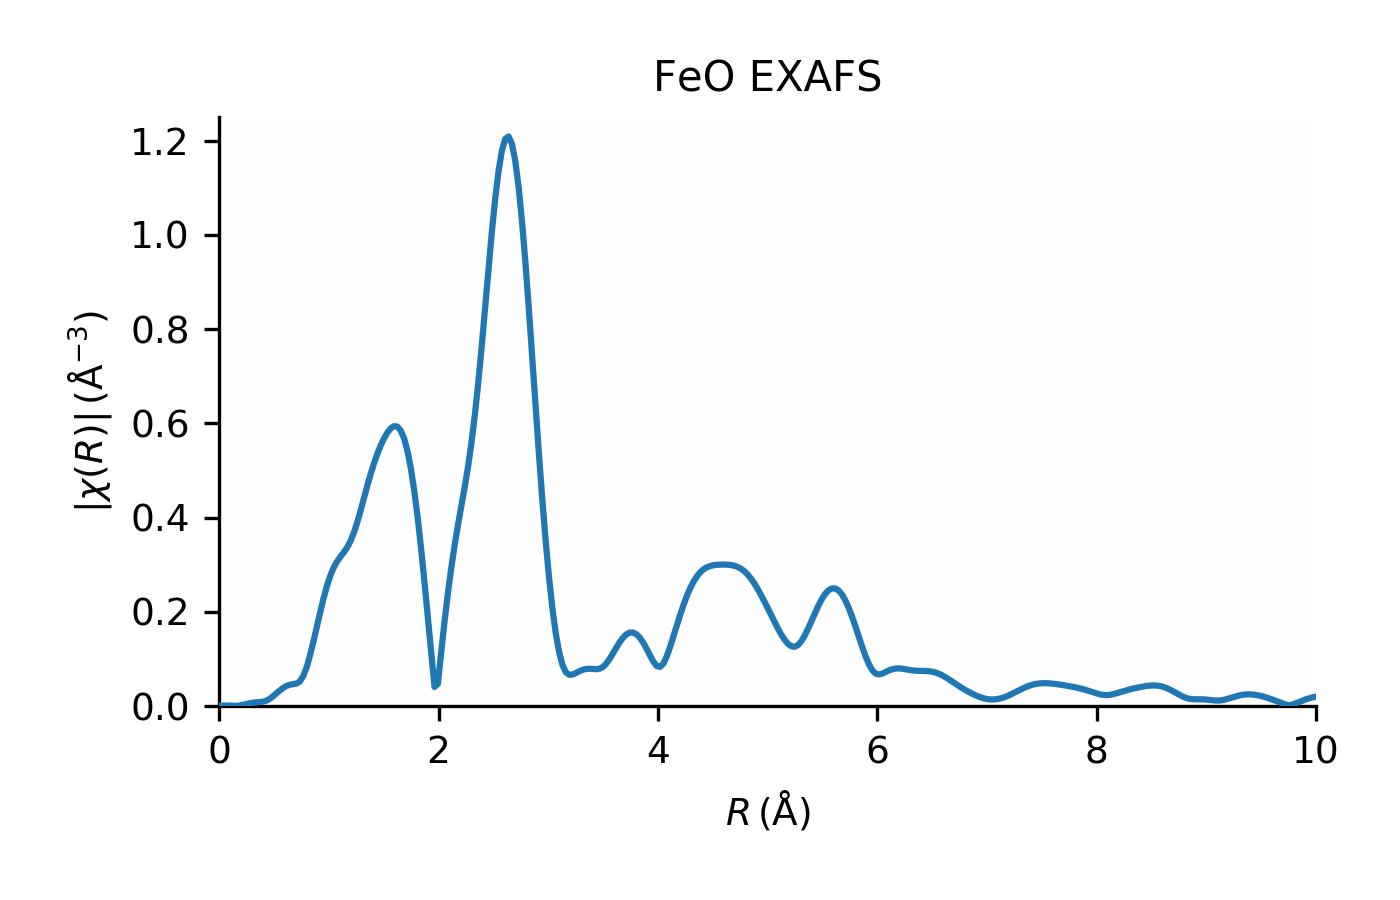
\includegraphics[width=60mm]{figs/errors/feo_chir}  }


  \end{column}
  \begin{column}[T]{60mm}

    {\onslide+<2-> 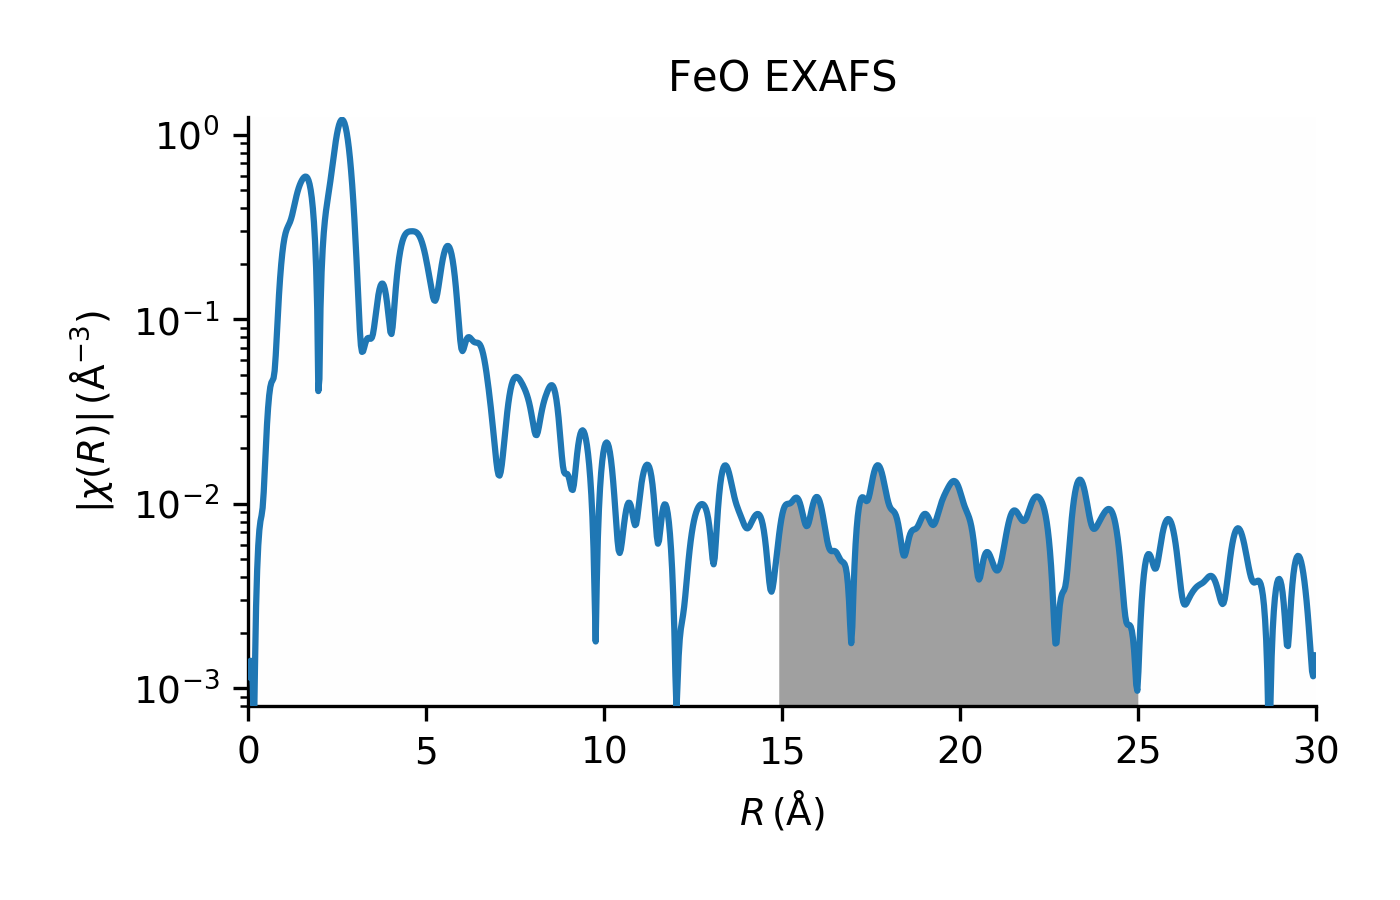
\includegraphics[width=60mm]{figs/errors/feo_chir_logscale} }

  \end{column}
\end{columns}

{\onslide+<2->

  \begin{cenpage}{105mm}


    The ``high-R'' portion of $\chi(R)$ can estimate the
    ``white noise'' in the data pretty well.

    \vmm
    This is easy to do, but we know it misses an important component:
  \end{cenpage}


  \begin{postitbox}{63mm}
      {uncertainties from  background subtraction}
  \end{postitbox}

}

\end{frame}


\begin{frame}\frametitle{ Uncertainties in $\chi(k)$ from background subtraction}


\vmm
\begin{cenpage}{105mm}

  We can propagate the uncertainties from the fit of the background spline
  to estimate the uncertainty in $\chi(k)$ from the background subtraction.

  \vmm \vmm

  This is {\BlueEmph{not white noise}}.   In fact, it tends to have a peak
  somewhat above $2 R_{\rm bkg}$
\end{cenpage}

\begin{columns}
  \begin{column}[T]{60mm}

    {\only<1> { 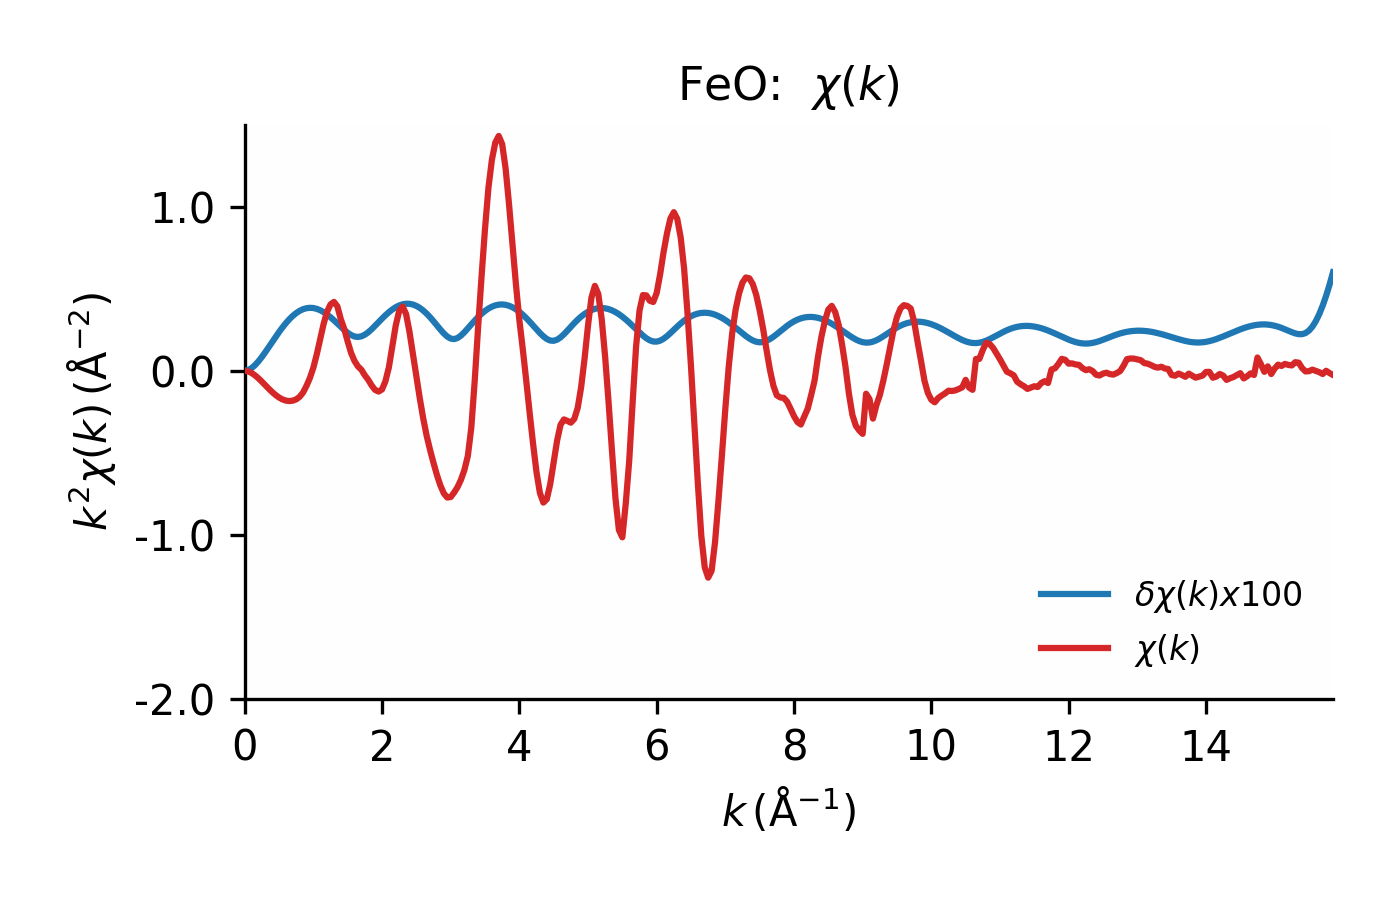
\includegraphics[width=60mm]{figs/errors/feo_chik_deltachi}}}

    {\only<2,3> { 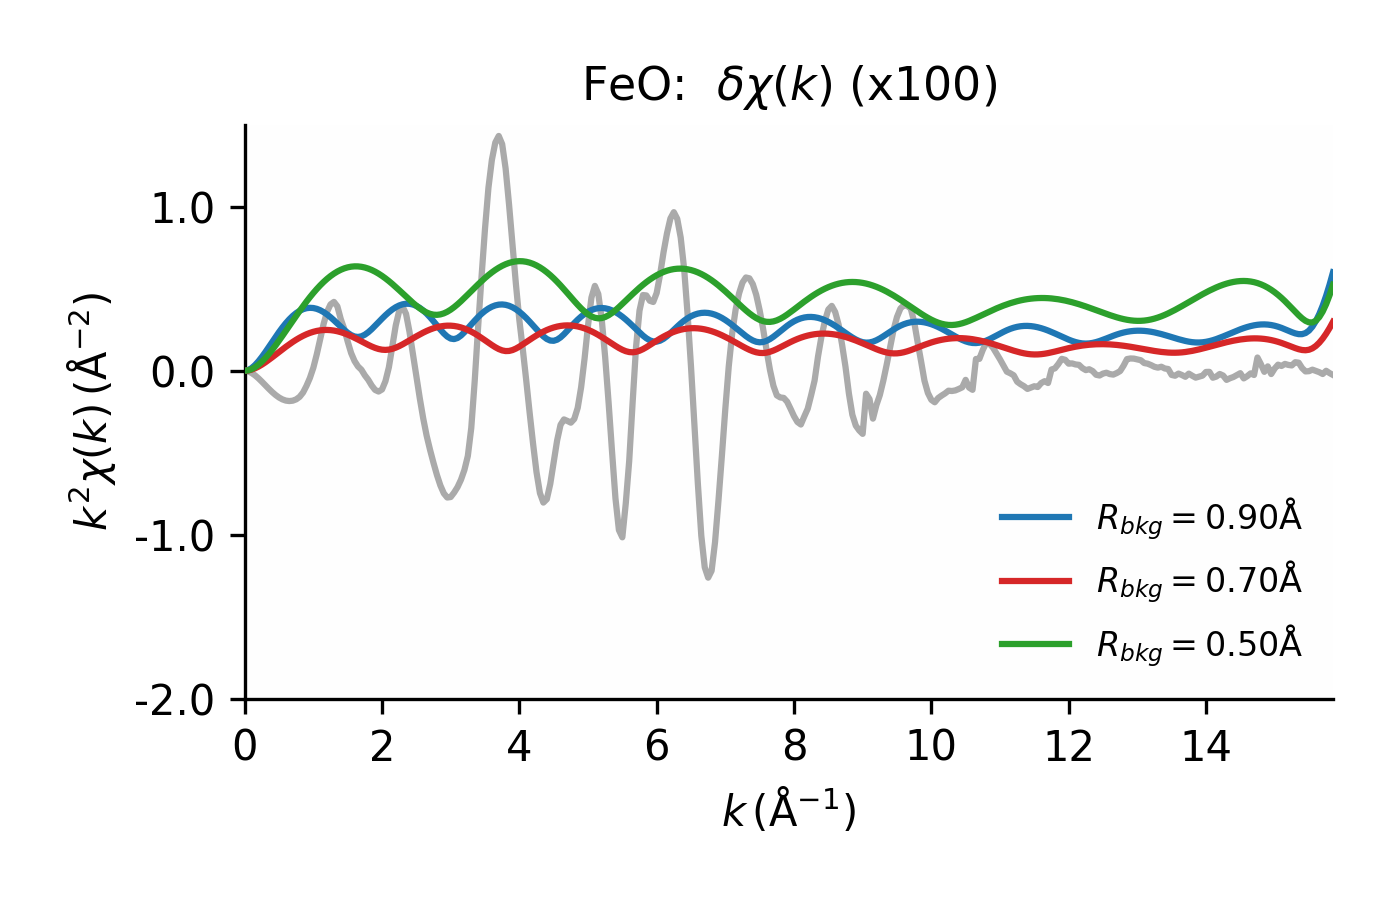
\includegraphics[width=60mm]{figs/errors/feo_deltachik_rbkg} }}

    \end{column}

    \begin{column}[T]{60mm}

      {\only<1>{ 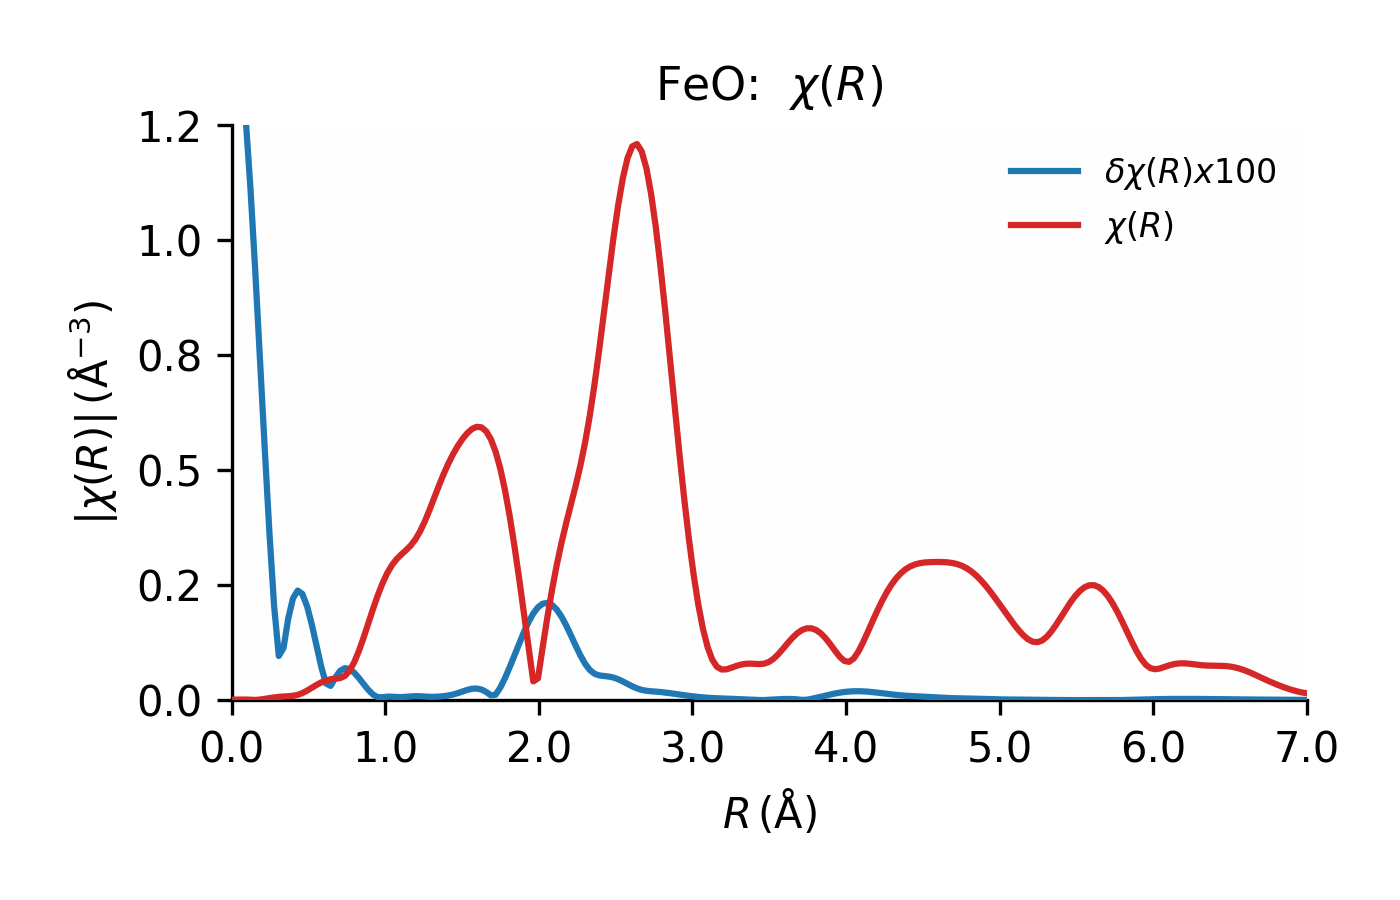
\includegraphics[width=60mm]{figs/errors/feo_chir_deltachi} }}

      {\only<2,3>{ 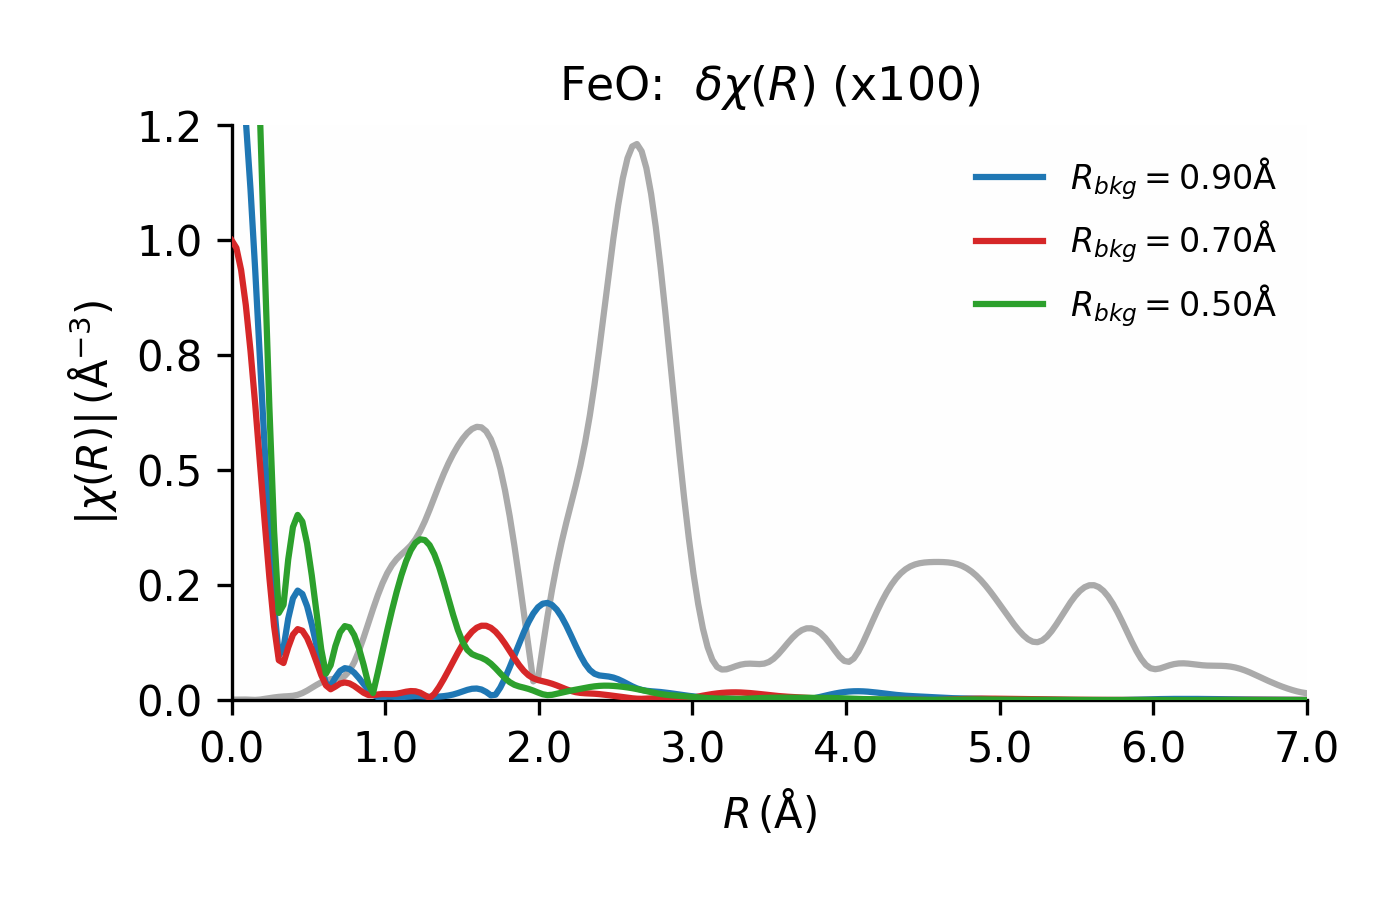
\includegraphics[width=60mm]{figs/errors/feo_deltachir_rbkg} }}

    \end{column}

\end{columns}

\vmm

{\onslide+<3-> {

\begin{cenpage}{105mm}

    Using this $\delta\chi(k)$ array reduces the $\chi^2$
    statistic by $2\times$ or  more.

\end{cenpage}

}}


\end{frame}

%%%%%%%%%%%%%%%%%%%%%%
\begin{slide}{Error Bars: the uncertainties in the fit variables}

\begin{cenpage}{95mm}
A fit finds a set of values $\Blue{x_0}$ that are the ``best fit'' of the variables
$\Blue{x}$ -- they give the lowest value of  $\chi^2$.

\begin{center} Uncertainties in $\Blue{x}$ are estimated by increasing the
  $\chi^2$ by 1: \end{center}

\end{cenpage}

\begin{columns}
\begin{column}{58mm}

\onslide+<2->

 \wpdf{58mm}{figs/errors/ellipse}

\end{column}
\begin{column}{55mm}

{\onslide+<2->
Some Parameters are {\RedEmph{Correlated}}:

\vmm

Changing {\Blue{$x$}} away from its best value will change the best value
for {\Blue{$y$}}.

\vmm

\begin{postitbox}{53mm}
  For EXAFS, ($R$, $E_0$) and ($N$, $\sigma^2$) are usually very highly
  correlated ($>0.85$).
\end{postitbox}
\vmm
}
\end{column}
\end{columns}

 \onslide+<2-> \vmm
 {\RedEmph{Increasing $\chi^2$ by 1 assumes we have a ``Good Fit'', with $\chi^2_\nu \approx 1$}}.

 \vmm We typically have  $\chi^2_\nu \gtrsim 50$  (Actually, we  {\emph{can
     now do better}}!).

\vmm
We increase the best $\chi^2$ by $\chi^2_\nu$ to estimate error bars.


\vmm \vmm

\end{slide}

% %%%%%%%%%%%%%%%%%%%%%%
% \begin{slide}{Error Bars: correlations between fit variables}


%     Pairs of variables can be {\RedEmph{correlated}}: changing one variable away
%     from its optimum value can be compensated by changing another variable away
%     from its best value.  The uncertainties needs to take correlations into
%     account.

%     \vmm\pause

%     \begin{center} \wpdf{50mm}{figs/errors/ellipse2}   \end{center}

%     \vmm
%     The uncertainty in $x$ is $\delta x$, NOT  $\delta x'$!

%     \vmm

%     The correlation between variables is given by the slope of the ellipse:

%     \begin{postitbox}{75mm}    how much does $y$ want to change when
%       changing $x$?
%     \end{postitbox}

%     \vmm

% \vfill
% \end{slide}

% \begin{slide}{Fitting in $R$- or $k$-space:  What do we model?}

  The $\chi^2$ definition didn't say anything about what our data
  $\chi_i^{\rm measured}$ actually is \ldots

  \onslide+<2->
  \vmm  We usually fit in $R$-space, so that  we can select which
  ``shells'' to ignore:

  \vmm \vmm

  \begin{columns}
    \begin{column}{53mm}  \wgraph{53mm}{reduction/chik}  \end{column}
    \begin{column}{53mm}  \wgraph{53mm}{reduction/chir_win}  \end{column}
  \end{columns}

  \vmm \onslide+<3-> Fitting $\chi(R)$ (both real and imaginary parts!) gives more
  meaningful fit statistics -- we know that we're not fitting all the
  spectral features.

  \vmm \onslide+<4->

  {\RedEmph{Plus:}}    We can have $\chi_i^{\rm measured}$  extend over

  \begin{center}{\Red{multiple data sets}}, {\Red{multiple $k$-weightings}},  etc, \end{center}

  as long as we generate the corresponding {\Red{$\chi_i^{\rm model}(x)$}} to
  match these data.

\vfill
\end{slide}


% 

\begin{slide}{EXAFS Analysis: Second Shell of FeO}

  Adding the 2nd shell Fe -- {\file{feffNNNN.dat}} for Fe-Fe -- and
  refining {\Blue{${R}$}}, {\Blue{${N}$}}, {\Blue{${\sigma^2}$}}:

    \vspace{1mm}

    \begin{tabular}{ll}
      \begin{minipage}{55mm} {\wpdf{54mm}{figs/fits/feo_r_2sh_mag}}
      \end{minipage}
      &
      \begin{minipage}{49mm}
        \vspace{1mm}

        ${|\chi(R)|}$ data for FeO (blue), and fit of ${\rm
          1^{st}}$ and ${\rm 2^{nd}}$ shells (red).  \vfill
        \vspace{1mm}

        These
        results are consistent with the known values for FeO:\par
         6 O at 2.14\AA, 12 Fe at 3.03\AA.
    \end{minipage}
  \end{tabular}

  \onslide+<2->{
  Fit results:     \hspace{6mm} Statistics: $R \approx 0.011 $
 \hspace{5mm}  $\chi^2_\nu \approx 4 $.

  \begin{center}
    \begin{tabular}{|c|rrrr|}
    \hline
    Shell & ${N}$ & ${R}$ (\AA) & ${\sigma^2}$
    (${\rm\AA^2}$) & ${\Delta E_0}$ (eV) \\
    \hline
    Fe-O  &  4.9(0.8) & 2.11(.01) & 0.011(.002) & {\Red{0.7(0.9)}}\\
    Fe-Fe & 11.6(1.4) & 3.07(.01) & 0.013(.002) & {\Red{0.7(0.9)}}\\
    \hline
  \end{tabular}
  \end{center}

  \vmm

  }
  \onslide+<3-> {
  These are typical even for a ``very good fit'' on known structures.

  The calculation for ${{\Red{f(k)}}}$ and
  ${{\Red{\delta(k)}}}$ are good, but not perfect!
}


\vfill
\end{slide}

\begin{slide}{EXAFS Analysis: Second Shell of FeO}

  Other views of the data and fit:

    \begin{tabular}{ll}
      \begin{minipage}{55mm} {\wpdf{55mm}{figs/fits/feo_k_2sh}}
      \end{minipage}
      &
      \begin{minipage}{53mm}  \setlength{\baselineskip}{11pt}
        The Fe-Fe EXAFS extends to higher-$k$ than the Fe-O EXAFS.

        \vmm Even in this simple system, there is some
        {\RedEmph{overlap}} of shells in ${R}$-space.

        {\onslide+<2->
          \vmm The fit in ${\rm Re[\chi(R)]}$ look especially
          good -- this is how the fits are done.

          \vmm
          }

    \end{minipage}
    \\
    \begin{minipage}{55mm}
      {\wpdf{55mm}{figs/fits/feo_r_2sh_paths}}
    \end{minipage}
    &
    \onslide+<2->{
      \begin{minipage}{55mm} {\wpdf{55mm}
          {figs/fits/feo_r_2sh_cmplx}}
      \end{minipage}}
  \end{tabular}

\vfill
\end{slide}

% 
\begin{slide}{Path Parameters: what can we vary in a fit?}

\begin{cenpage}{108mm}
  The EXAFS Equation has at least 4 adjustable parametes {\RedEmph{Per
      Path}}:
  $E_0$, $NS_0^2$, $R$, and $\sigma^2$.  \hspace{5mm}     But $N_{\rm idp}$  is low:

  \[ N_{\rm idp} = 8 \> \> \>
  {\rm for} \> \Delta R = 1 \, {\rm \AA} \>\> {\rm and} \>\> \Delta k = 12.5\,
  {\rm \AA^{-1} } \]

  \vmm\onslide+<2->

  For simple crystalline structures with well-isolated, single-scattering
  path (like FeO), it's OK to fit $N$, $R$, $\sigma^2$, and $E_0$ for every
  path.

  \vmm

  For more complicated problems, we need a way to limit the number of
  parameters varied.

  \vmm

  We might {\emph{want}} to impose relationships between parameters to get
  more meaningful results\ldots


\end{cenpage}
\vfill
\end{slide}



% \subsection{Constraints and Generalized Variables}
\begin{frame}[fragile] \frametitle{Constraints and Generalized Variables}

  Instead of varying the Path Parameters directly, we write them in terms of
  {\RedEmph{Generalized Variables}}.  This allows simple {\RedEmph{Constraints}} and model building:

\begin{columns}
  \begin{column}{53mm}

  \begin{CodeBlock}{50mm}{Parameter=Variable}
{\Blue{\# one variable e0 for 2 paths}}
{\Red{params = group(e0 = guess(1.0), \ldots)}}

path1  = feffpath('feo.dat', {\Red{e0='e0'}})
path2  = feffpath('fefe.dat', {\Red{e0='e0'}})
  \end{CodeBlock}
  \hspace{1mm}   \vmm

  \onslide+<2->
  \begin{CodeBlock}{50mm}{Mixed Coordination Shell}
{\Blue{\# mix O and S in 1st coordination shell}}
params = group(s02   = param(0.80, vary=False),
               sfrac = guess(0.5))

path1 = feffpath('feo.dat', {\Red{s02='s02*sfrac'}})
path2 = feffpath('fes.dat', {\Red{s02='s02*(1-sfrac)'}})
  \end{CodeBlock}

  \vmm

  \end{column}
  \begin{column}{57mm}
    \onslide+<3->
  \begin{CodeBlock}{55mm}{Einstein Temperature }
{\Blue{\# Use 1 ``theta'' to set sigma2 for multiple paths}}

params = group(amp=param(1, vary=True),
               theta=param(250, min=0, vary=True), \ldots)

path1_100K = feffpath('fefe.dat', s02='amp', \ldots,
                      sigma2='sigma2_eins(100, theta)')

path1_200K = feffpath('fefe.dat', s02='amp', \ldots,
                      sigma2='sigma2_eins(200, theta)')

path1_300K = feffpath('fefe.dat', s02='amp', \ldots,
                      sigma2='sigma2_eins(300, theta)')

  \end{CodeBlock}\\
\end{column}
\end{columns}

\vmm This allows us to use {\BlueEmph{Prior  Knowledge}} into the data analysis, and
consider more complicated problems:

\vfill

  \begin{itemize}
  \item force one $R$ for the same bond for data taken from different
    edges.

  \item model complex distortions (height of a sorbed atom above a surface).
  \end{itemize}


\end{frame}

% \begin{slide}{Constraints, Generalized Variables examples}


%   Constraints and Generalized Variables are one kind of ``Prior
%   Knowledge'',  allowing us to build and compare simple physical models for
%   our data.

%   \vmm   This allows us to consider more complicated problems:

%   \vmm

%   {\Red{
%       \begin{tabular}{clcl}
%         &multiple neighboring species  &&  multiple sites for central atom \\
%         &multiple scattering paths     &&  multiple polarizations \\
%         &multiple data sets            &\hspace{4mm}&  multiple edges to co-refine   \\
%       \end{tabular}
%     }}

%   \vmm Other constraints:

%   \begin{itemize}
%   \item force one $R$ for the same bond for data taken from different
%     edges.

%   \item model complex distortions (height of a sorbed atom above a surface).
%   \end{itemize}

% \vfill
% \end{slide}

% 
%%%%%%%%%%%%%%%%%%%%%%
\subsection{Example: Cu metal at 3 temperature}
\begin{frame}[fragile] \frametitle{Example: Cu metal at 3 temperature}


    A very simple example of a Multi-Data-Set Fit:

    Cu metal, at 3 different  temperatures: 10K, 50K 150K.

   \begin{columns}
     \begin{column}{48mm}
        \vmm  Path Parameters:
       \begin{itemize}
       \item $E_0$:  Same for all $T$
       \item $S_0^2$  Same for all $T$
       \item $R$:  expands linearly with $T$ (slope + offset).
       \item $\sigma^2$:  goes as Einstein temperature (as before).
       \end{itemize}

       {\RedEmph{12 parameters become 5.}}

       \vmm Fit range: \vmm

       \hspace{2mm} $R = [1.60, 2.75] \rm\, \AA$

       \vmm
       \hspace{2mm}  $k = [1.50, 18.50] \rm\, \AA^{-1}$
     \end{column}
     \begin{column}{53mm}

  \begin{CodeBlock}{55mm}{Cu at three temperatures}

# define fitting parameter group
pars = group(amp      = param(1, vary=True),
             del_e0   = guess(2.0),
             theta    = param(250, min=10, vary=True),
             dr_off   = guess(0),
             dr_slope = guess(0) )

# define 3 Feff Path, give expressions for Path Parameters
path1_10  = feffpath('feff0001.dat',
                     s02='amp', e0='del_e0',
                     deltar='dr_off + 10*dr_slope',
                     sigma2='sigma2_eins(10, theta)')

path1_50  = feffpath('feff0001.dat',
                     s02='amp', e0='del_e0',
                     deltar='dr_off + 50*dr_slope',
                     sigma2='sigma2_eins(50, theta)')

path1_150 = feffpath('feff0001.dat',
                     s02='amp', e0='del_e0',
                     deltar='dr_off + 150*dr_slope',
                     sigma2='sigma2_eins(150, theta)')

   \end{CodeBlock}
 \end{column}
\end{columns}

\end{frame}


%%%%%%%%%%%%%%%%%%%%%%
\subsection{Example: Cu metal Results}
\begin{frame}[fragile] \frametitle{Example: Cu metal Results}

  \begin{tabular}{ll}
    \begin{minipage}{50mm}
      \begin{tabular}{lll}
        {\ } &{\tt{amp}}  &   $0.91(0.08)$ \\
        &{\tt{theta}}  &   $233.5(19.6) \rm\, K $ \\
        &{\tt{del\_e0}}  &   $0.4(1.3) \rm \, eV$ \\
        & {\tt{dr\_off}} &   $0.002(0.003) \rm \, {\AA}/K $ \\
        &{\tt{dr\_slope}}   &    $0.5(1.8)\times 10^{-5} \rm \, {\AA}$ \\
      \end{tabular}
  \vmm
\end{minipage} &
\begin{minipage}{50mm}
  \wpdf{49mm}{figs/Cu3temp/cu_3temp_mag10}
\end{minipage} \\
\begin{minipage}{50mm}
  \wpdf{49mm}{figs/Cu3temp/cu_3temp_50}
\end{minipage} &
\begin{minipage}{50mm}
  \wpdf{49mm}{figs/Cu3temp/cu_3temp_150}
\end{minipage}\\
\end{tabular}
\end{frame}

%%%%%%%%%%%%%%%%%%%%%%
% \begin{slide}{Room Temperature Cu Fit }

%   Simple fit to first shell of Cu foil (300K): $k = [2,16] \rm\,
%     \AA^{-1}$, $R = [1.7,2.6] \rm\, \AA$, $k$-weight=2, $N_{\rm idp} = 8.4
%     $.  Fit results and statistics:


%     {
%       \hspace{0.1mm}\begin{tabular}{lll}
%         $R = 2.548(0.007) \, \rm\AA$
%         &
%         $\Delta E_0 = 4.5(0.6)$
%         &
%         $C_3      = 9(9) \times10^{-5} \rm\, \AA^3$
%         \\
%         $\epsilon_k = 1.6 \times 10^{-4}$
%         &
%         $S_0^2 = 0.96(0.04)$
%         &
%         $\sigma^2 = 8.5(0.3) \times10^{-3} \rm\, \AA^2$
%         \\
%         $\chi^2 = 678$ &
%         $\chi^2_\nu = 196.7$   & ${\cal{R}} = 0.00107 $\\
%       \end{tabular}
%     }

%     \vmm
%       \begin{tabular}{lcl}
%         \wgraph{49mm}{errors/cufit02} & \hspace{2mm} &
%         \wgraph{49mm}{errors/cufit01} \\
%       \end{tabular}

%       \begin{itemize}
%       \item ${\cal{R}} = 0.1\% $ -- a good fit!  But like $\chi^2_\nu$,
%         ${\cal{R}}$ is larger than the $\epsilon_k$ suggests.
%       \item These error bars account for correlations.  They increase
%         $\chi^2$ by $\chi^2_\nu$ (not 1), which scales them by
%         $\sqrt{\chi^2_\nu}\approx 14$ over ``increase $\chi^2$ by 1''.
%       \end{itemize}

%       \vmm
% \vfill
% \end{slide}

% 

\begin{slide}{The EXAFS Equation: Recap}


  \begin{cenpage}{120mm}

    Even with all those complications and caveats, we still use the
    {\BlueEmph{EXAFS Equation}}: \vspace{-1mm}

  \begin{center}
    \[ \chi(k) = \sum_j {\frac{{\Blue{N_j}} {\Red{f_j(k)}}
        e^{-2{\Blue{R_j}}/{\Red{\lambda(k)}}}
        e^{-2k^2{\Blue{\sigma_j^2}}}}{k{\Blue{R_j}}^2}
      {\sin[{2k{\Blue{R_j}} + {\Red{\delta_j(k)}}] }}} \]
  \end{center}

  \vmm

  where $\Red{f(k)}$ and $\Red{\delta(k)}$ are
  {\RedEmph{photo-electron scattering properties}} of the neighboring
  atom and $ \Red{\lambda(k)} $ is the photo-electron mean-free-path.

  \vmm


  \vmm
Again, if we know these properties, we can determine:
  \onslide+<2->
    \begin{description}
      \settowidth{\labelwidth}{15mm}
      \setlength{\itemindent}{15mm}
      \setlength{\leftmargin}{15mm}
    \item[$R$] distance to neighboring atom.
    \item[$N$] coordination number of neighboring atom.
    \item[$\sigma^2$] mean-square disorder of neighbor distance \par
      \hspace{13.5mm} (or
      more complicated disorder terms).
    \end{description}

  \vmm
  \onslide+<3>
  ${\Red{f(k)}}$ and ${\Red{\delta(k)}}$ depend on atomic number
  {\BlueEmph{Z}} of the scattering atom, so we can also determine the
  species of the neighboring atom.

\end{cenpage}

\end{slide}


\begin{slide}{EXAFS Theory:  Conclusions}
  
  \begin{cenpage}{110mm}
    We have an EXAFS Equation that we can use to model EXAFS data.

  \begin{center}
    \[ \chi(k) = \sum_j {\frac{{\Blue{N_j}} {\Red{f_j(k)}}
        e^{-2{\Blue{R_j}}/{\Red{\lambda(k)}}}
        e^{-2k^2{\Blue{\sigma_j^2}}}}{k{\Blue{R_j}}^2}
      {\sin[{2k{\Blue{R_j}} + {\Red{\delta_j(k)}}] }}} \]
  \end{center}

  \vmm
  In later videos and demos we'll show how to use this for
  analyzing EXAFS data.

  

  \vmm\vmm \hrule \vmm
  
  More information on X-rays and X-ray Absorption Spectroscopy:

  \begin{itemize}
  \item[] {\Blue{https://xafs.xrayabsorption.org/}}
  \item[] {\BlueEmph{Fundamentals of XAFS}} M. Newville, Reviews in  Mineralogy \& Geochemistry {\bf{78}}, 2014.
  \item[] {\BlueEmph{Introduction to XAFS}} G. Bunker, Cambridge Univ  Press,  2010.
  \item[] {\BlueEmph{XAFS for Everyone}} S. Calvin, CRC Press, 2013.
  \item[]  {\BlueEmph{Elements of Modern X-ray Physics}}  J.~Als-Nielsen
    \& D.~McMorrow,  John Wiley \& Sons. 2001
    
  \end{itemize}

\end{cenpage}


 \vfill
\end{slide}
 





\begin{slide}{Using FEFF for EXAFS Analysis}


  \begin{cenpage}{126mm}

    Using {\feff} to calculate the scattering factors does not need to be
    too hard.

    \begin{itemize}
    \item   Start with a crystal structure that close to your structure.
    \item   Make sure you have the absorbing element and edge right!
    \item    Pay attention to the {\RedEmph{degeneracy}}, or coordination number for    each path.
    \item    Don't be afraid to alter the atoms list in {\feffinp}, especially    replacing atom types or importing structures from simulations.
    \item    Don't be afraid to mix paths from different calculations.
    \item   Don't worry too much about the rest of it -- let the GUI programs    ({\xasviewer}, {\artemis}) help you manage these calculations.
    \end{itemize}

        \vmm     \hrule \vmm

  More information on X-rays and X-ray Absorption Spectroscopy:

  \begin{itemize}
  \item[] {\Blue{https://xafs.xrayabsorption.org/}}
  \item[] {\BlueEmph{Fundamentals of XAFS}} M. Newville, Reviews in  Mineralogy \& Geochemistry {\bf{78}}, 2014.
  \item[] {\BlueEmph{Introduction to XAFS}} G. Bunker, Cambridge Univ  Press,  2010.
  \item[] {\BlueEmph{XAFS for Everyone}} S. Calvin, CRC Press, 2013.
  \item[]  {\BlueEmph{Elements of Modern X-ray Physics}}  J.~Als-Nielsen
    \& D.~McMorrow,  John Wiley \& Sons. 2001

  \end{itemize}

\end{cenpage}


 \vfill
\end{slide}



\end{document}
